\documentclass[aspectratio=169]{beamer}

% Required packages
\usepackage{graphicx}
\usepackage{booktabs}
\usepackage{ragged2e}
\usepackage{hyperref}
\usepackage{color, xcolor}
\usepackage{amsmath} 
\usepackage{setspace} 

\definecolor{NavyBlue}{RGB}{18, 28, 97}
\definecolor{CyberTeal}{RGB}{0, 130, 130}
\definecolor{SecurityGreen}{RGB}{67, 160, 71}
\definecolor{AlertOrange}{RGB}{251, 140, 0}
\definecolor{DangerRed}{RGB}{229, 57, 53}
\definecolor{DarkGrayText}{RGB}{60, 60, 60}

\usetheme{metropolis}

\setbeamercolor{frametitle}{fg=white, bg=NavyBlue}
\setbeamercolor{section title}{fg=NavyBlue}
\setbeamercolor{subsection title}{fg=CyberTeal}
\setbeamercolor{structure}{fg=NavyBlue}
\setbeamercolor{item}{fg=DarkGrayText}
\setbeamercolor{itemize item}{fg=SecurityGreen}
\setbeamercolor{itemize subitem}{fg=CyberTeal}
\setbeamercolor{itemize subsubitem}{fg=NavyBlue}
\setbeamercolor{block title}{fg=white, bg=CyberTeal}
\setbeamercolor{block body}{bg=white!95!NavyBlue!10}
\setbeamercolor{alert block title}{fg=white, bg=DangerRed}
\setbeamercolor{alert block body}{bg=white!95!DangerRed!10}
\setbeamercolor{normal text}{fg=DarkGrayText}
\setbeamercolor{title page header}{fg=NavyBlue}

\setbeamerfont{normal text}{size=\small} 
\linespread{1.15} 

\usepackage{etoolbox}
\pretocmd{\tableofcontents}{\vspace{1em}}{}{}
\apptocmd{\tableofcontents}{\vspace{1em}}{}{}

\title{Password Security Checker\\Browser Extension}
\author{Team Members: \newline Imene Fatma DJELILI \\
\and Hadil HATTABI \\
\and Firdaws BASSAID \\
\and Hachem Safi Eddine SEKHSOUKH \\
\and Youcef GUERGOUR \\
\and Rafik MESSAOUD NACER}
\institute{National higher school of artificial intelligence (ENSIA)}
\date{\today}
\logo{
\includegraphics[height=1cm]{EnsiaLogo.png}}

\begin{document}

\begin{frame}
  \titlepage
\end{frame}

\begin{frame}{Outline}
  \vspace{0.5em} 
  \tableofcontents
  \vspace{0.5em} 
\end{frame}

\section{Introduction}
\begin{frame}{Introduction: Securing the Digital Frontier}
  \begin{itemize}
    \item \textbf{The Challenge:} Vulnerability of online accounts due to weak, reused, or breached passwords.
    \begin{itemize}
      \item Common user practices (reuse, weak choices)
      \item Threat landscape (credential stuffing, brute-force, phishing)
    \end{itemize}
    \item \textbf{The Solution: Password Security Checker}
    \begin{itemize}
       \item Intelligent, cross-browser web extension.
       \item Real-time feedback and enforcement on password forms.
       \item Empowers users to improve password hygiene.
    \end{itemize}
  \end{itemize}
\end{frame}

\section{Objectives}
\begin{frame}{Core Objectives}
  \begin{itemize}
    \item \textbf{Real-time Analysis \& Enforcement:} Assess and block weak passwords instantly.
    \item \textbf{Comprehensive Vulnerability Assessment:} Identify risks from patterns, reuse, and public breaches.
    \item \textbf{Intuitive User Guidance:} Provide clear feedback via UI and notifications.
    \item \textbf{Broad Browser Accessibility:} Ensure consistent functionality across major browsers.
    \item \textbf{Promote Security Best Practices:} Educate users through integrated tips.
  \end{itemize}
\end{frame}

\section{Key Features}

\subsection{Real-time Strength Assessment}
\begin{frame}{Key Feature: Real-time Assessment \& Enforcement}
  \begin{columns}
    \column{0.5\textwidth}
    \begin{itemize}
      \item Dynamic feedback while typing in password fields.
      \item Visual status indicators (color-coded icon).
      \item Detailed tooltip explanations and suggestions.
      \item Evaluation metrics:\\ Length, Complexity, Entropy, Common Patterns.
      \item \textbf{Enforcement:} Prevent submission of passwords failing minimum security criteria.
    \end{itemize}
    \column{0.5\textwidth}
    \centering
    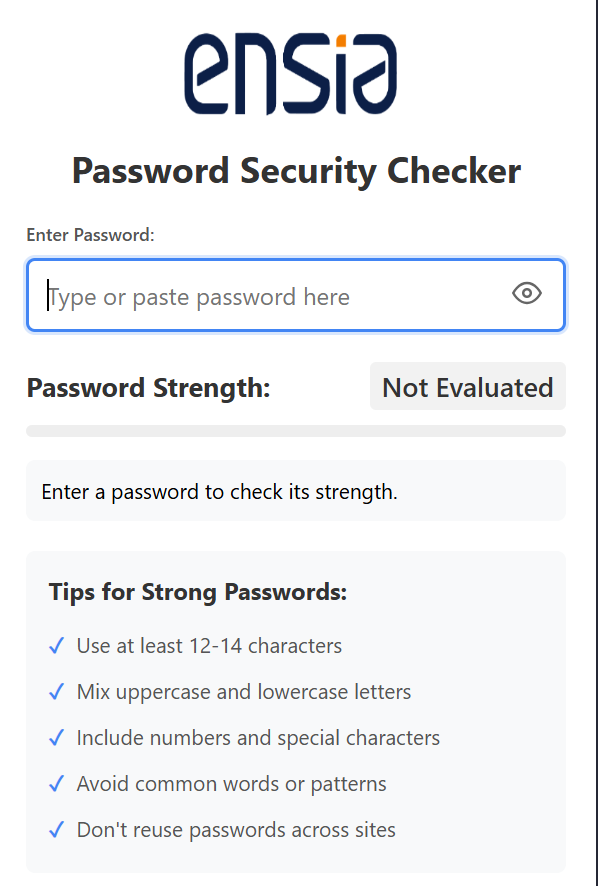
\includegraphics[width=0.8\textwidth]{type.png}
  \end{columns}
\end{frame}

\begin{frame}{Key Feature: Real-time Assessment Statuses}
  \centering
  \begin{tabular}{cc}
      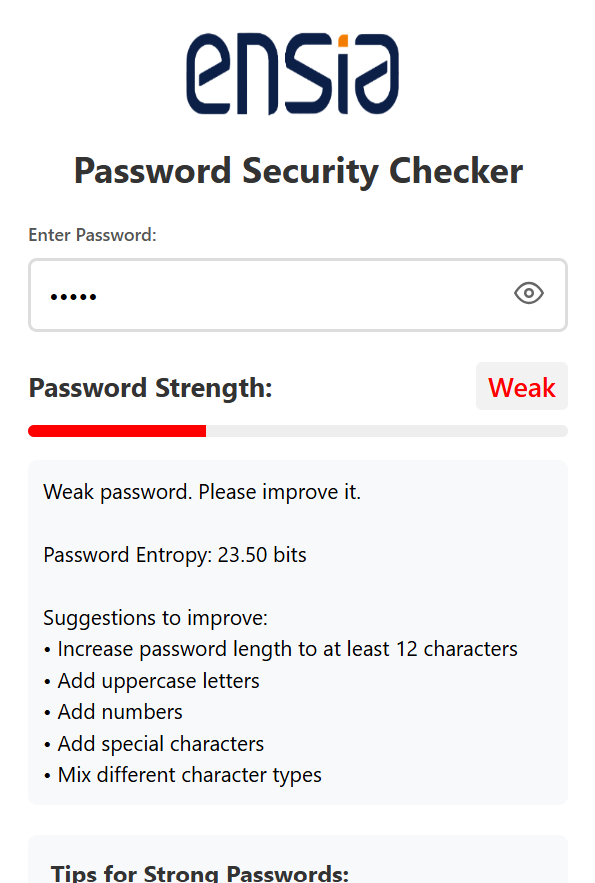
\includegraphics[width=0.4\textwidth]{low.png} &
      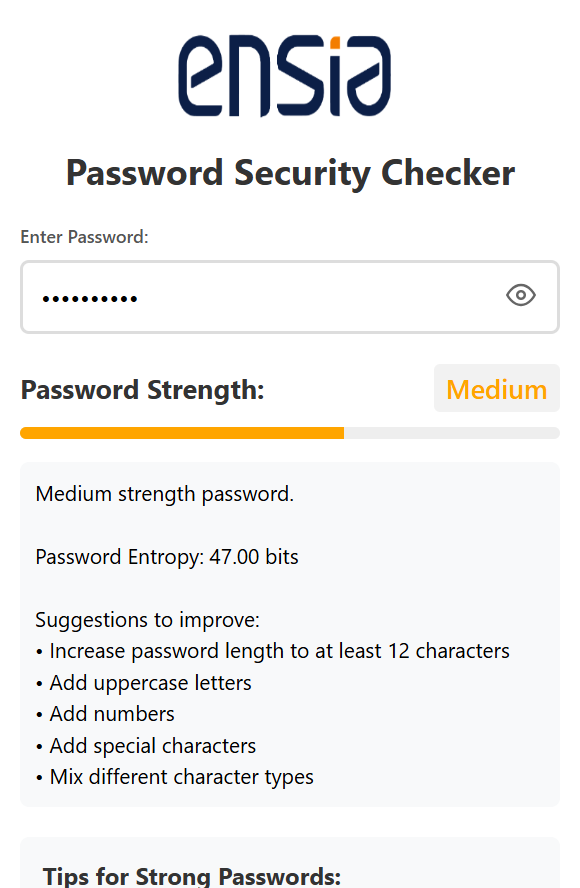
\includegraphics[width=0.4\textwidth]{medium.png} \\
      \small Low Strength & \small Medium Strength \\[1em]
      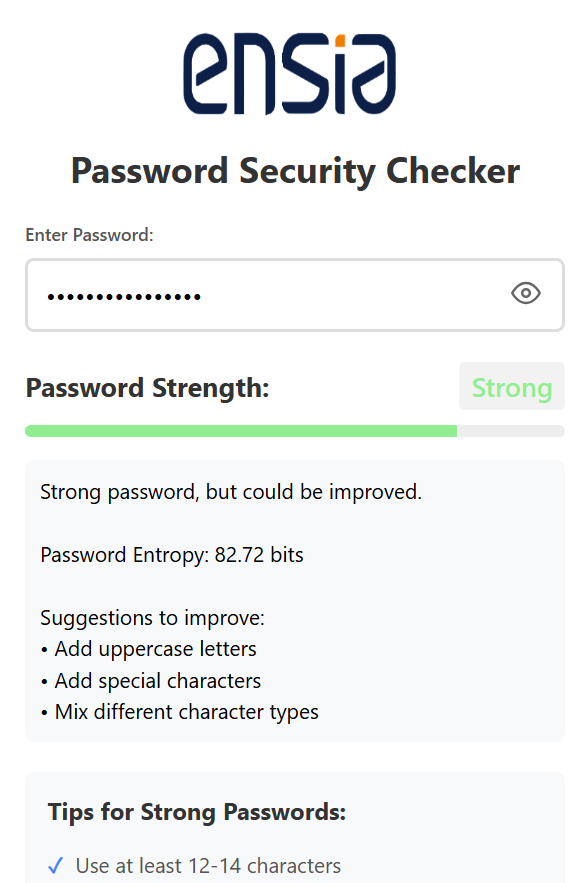
\includegraphics[width=0.4\textwidth]{strong.png} &
      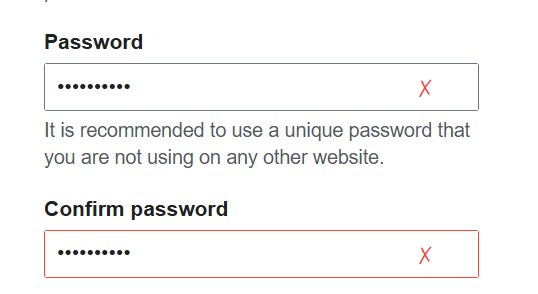
\includegraphics[width=0.4\textwidth]{red.png} \\
      \small Strong Strength & \small Weak/Blocked Submission \\
  \end{tabular}
\end{frame}

\subsection{Password Reuse Detection}
\begin{frame}{Key Feature: Password Reuse \& Breach Detection}
  \begin{columns}
    \column{0.5\textwidth}
    \begin{itemize}
      \item \textbf{Local Reuse Check:}
      \begin{itemize}
        \item Detects if the password (hashed) was seen on other visited sites.
        \item Provides list of previously used domains.
      \end{itemize}
      \item \textbf{Global Breach Check:}
      \begin{itemize}
        \item Secure query to Have I Been Pwned (HIBP) API.
        \item Uses privacy-preserving k-anonymity (sends hash prefix).
        \item Reports breach count if password found in public data.
      \end{itemize}
    \end{itemize}
    \column{0.5\textwidth}
    \centering
    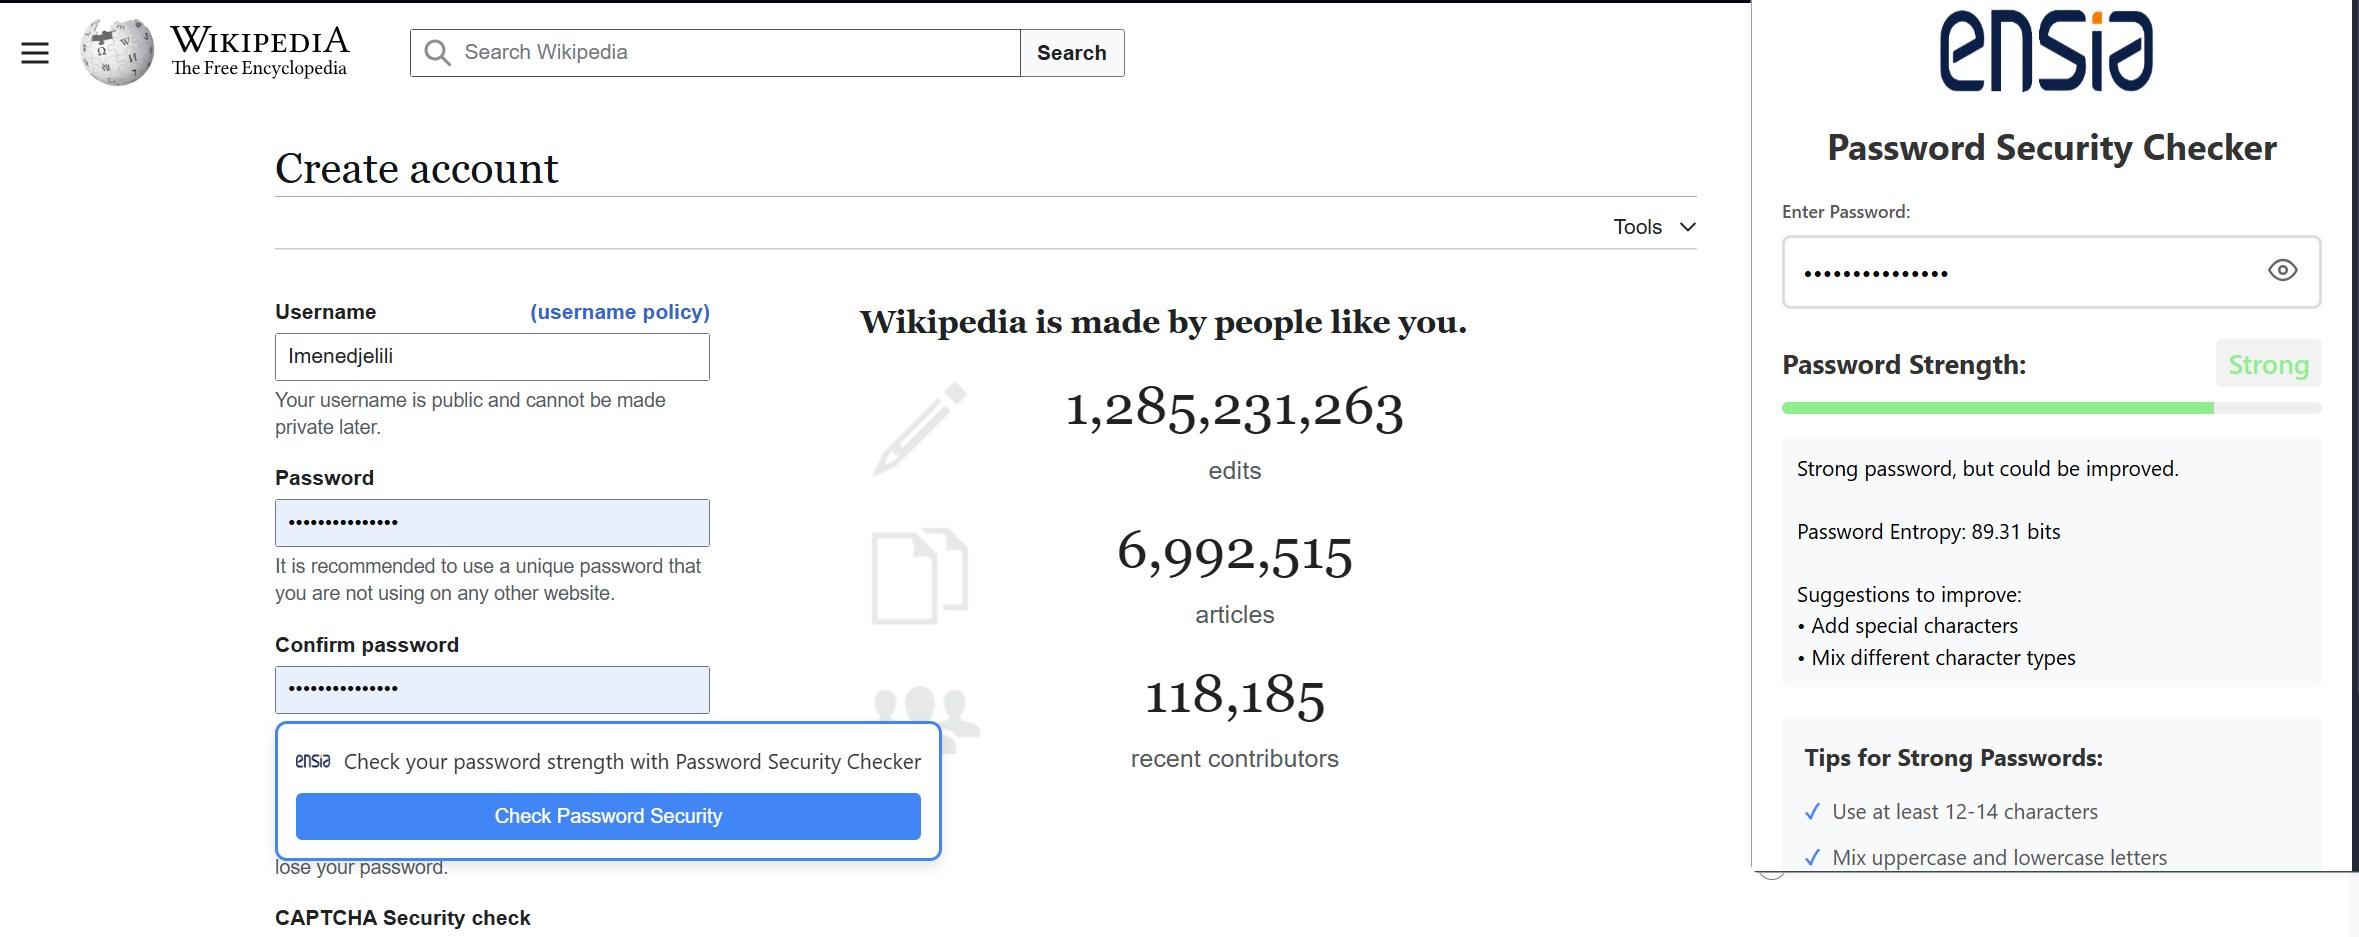
\includegraphics[width=0.8\textwidth]{checker.png}
  \end{columns}
\end{frame}

\subsection{Cracking Simulation}
\begin{frame}{Key Feature: Local Cracking Simulation \& Alerts}
  \begin{columns}
     \column{0.5\textwidth}
      \begin{itemize}
        \item \textbf{Simulates Common Attacks:}
        \begin{itemize}
          \item Dictionary and common patterns.
          \item Character substitutions, keyboard patterns.
          \item Date formats.
        \end{itemize}
        \item Estimates theoretical offline cracking time.
        \item \textbf{Critical Notifications:}
        \begin{itemize}
           \item Immediate browser notification for easily "crackable" or breached passwords.
           \item Periodic reminders for unaddressed vulnerabilities.
        \end{itemize}
     \end{itemize}
      \column{0.5\textwidth}
      \centering
      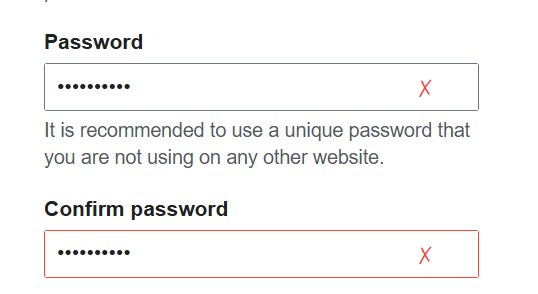
\includegraphics[width=0.8\textwidth]{red.png}
  \end{columns}
\end{frame}

\subsection{Branding Integration}
\begin{frame}{Key Feature: ENSIA Branding}
  \begin{columns}
     \column{0.5\textwidth}
     \begin{itemize}
       \item Integrated ENSIA logo in user interface elements:
       \begin{itemize}
         \item Popup interface.
         \item Inline notifications/tips.
       \end{itemize}
       \item Reinforces authenticity and trust.
       \item Aligns with the project's academic context.
     \end{itemize}
     \column{0.5\textwidth}
     \centering
     
\includegraphics[height=2cm]{EnsiaLogo.png}
  \end{columns}
\end{frame}

% Architecture
\section{Technical Overview}
\begin{frame}{Architecture \& Implementation Highlights}
  \begin{itemize}
    \item \textbf{Standard Browser Extension Model:}
    \begin{itemize}
       \item Background Script: Core logic, state, external API calls.
       \item Content Script: DOM interaction, UI injection, event listeners.
       \item Popup Script: On-demand user interface.
    \end{itemize}
    \item \textbf{Cross-Browser Compatibility:}
    \begin{itemize}
      \item Uses a polyfill (`browser-polyfill.js`) for unified API access.
      \item Supports different manifest versions (V2/V3).
      \item Automated build process for browser-specific packages.
    \end{itemize}
     \item \textbf{Data Handling:} Secure local storage of hashed passwords for history/tracking.
     \item \textbf{Resources:} Local data files (e.g., common passwords CSV).
  \end{itemize}
\end{frame}

\section{Evaluation \& Testing}
\begin{frame}{Evaluation \& Testing Summary}
  \begin{itemize}
    \item \textbf{Functional Testing:} Verified all key features (real-time analysis, enforcement, reuse/breach checks, notifications) on various websites and forms.
    \item \textbf{Cross-Browser Testing:} Confirmed consistent behavior and functionality across Chrome, Firefox, Edge, and Safari builds.
    \item \textbf{Reliability Tests:} Addressed edge cases (e.g., network issues for HIBP, dynamic forms via `MutationObserver`).
    \item Project demonstrates robust password security evaluation and user alerting capabilities across target platforms.
  \end{itemize}
\end{frame}

\section{Strengths and Limitations}
 \begin{frame}{Strengths}
   \begin{itemize}
     \item Comprehensive Real-time Analysis
     \item Proactive Enforcement
     \item Timely Critical Alerts via Browser Notifications
     \item Strong Cross-Browser Compatibility
     \item Privacy-Respecting Breach Check (HIBP k-anonymity)
     \item Secure Local Storage (Hashed Passwords)
     \item Intuitive User Interface and Experience
     \item Self-Contained Local Cracking Simulation
     \item ENSIA Branding Integration
   \end{itemize}
 \end{frame}

 \begin{frame}{Limitations}
   \begin{itemize}
     \item HIBP checks require active internet connection.
     \item Potential for minor UI conflicts on highly complex web pages.
     \item Limited user configuration options in current version.
     \item Cracking time estimates are theoretical offline speeds.
   \end{itemize}
 \end{frame}

\section{Future Work}
\begin{frame}{Future Enhancements}
  \begin{itemize}
    \item Enhanced Offline Capability (Local breach data caching).
    \item Machine Learning Integration for adaptive prediction.
    \item Configurable Security Policies via Options Page.
    \item Improved UI/UX and notification methods.
    \item Contextual Educational Tips based on detected weaknesses.
    \item Security Audit Integrations (anonymized reporting - requires backend).
    \item Expansion of Local Simulation Attacks.
    \item Preparation for Official Store Publication.
  \end{itemize}
\end{frame}

% Resources
 \section{Resources \& Technologies}
 \begin{frame}{Key Resources \& Technologies}
   \begin{itemize}
     \item Have I Been Pwned (HIBP) API (\url{https://haveibeenpwned.com/API/v3})
     \item Browser Extension Developer Documentation (Chrome, Firefox, Safari)
     \item \href{https://github.com/mozilla/webextension-polyfill}{\texttt{webextension-polyfill}} library
     \item \href{https://www.papaparse.com/}{PapaParse} (CSV parsing)
     \item OWASP Foundation \& NIST SP 800-63B (Security Guidelines)
   \end{itemize}
 \end{frame}

\section{Links}
\begin{frame}{Project Links}
  \begin{itemize}
    \item \textbf{GitHub Repository:} \url{https://github.com/imenedjelili/CNS-Project---Secondary}
    \item \textbf{Demo Video:} \url{https://drive.google.com/drive/folders/1MTh8wgICNQBM3qrUc3JF0slHRFNU7VEn?usp=sharing} 
  \end{itemize}
  \vspace{1em}
\end{frame}

\begin{frame}{Thank You / Questions?}
   \centering
   \vspace*{1cm}
   {\Huge Thank You!}
   \vfill
   {\Large Questions?}
   \vfill
   \small Contact: \newline
   fatma.imene.djelili@ensia.edu.dz, hadil.hattabi@ensia.edu.dz, \newline
   firdaws.bassaid@ensia.edu.dz, hachem.safi.eddine.sekhsoukh@ensia.edu.dz, \newline
   youcef.guergour@ensia.edu.dz, rafik.messaoud.macer@ensia.edu.dz
\end{frame}

\end{document}